%%%%%%%%%%%%%%%%%%%%%%%%%%%%%%%%%%%%%%%%%
% Jacobs Landscape Poster
% LaTeX Template
% Version 1.1 (14/06/14)
%
% Created by:
% Computational Physics and Biophysics Group, Jacobs University
% https://teamwork.jacobs-university.de:8443/confluence/display/CoPandBiG/LaTeX+Poster
% 
% Further modified by:
% Nathaniel Johnston (nathaniel@njohnston.ca)
%
% This template has been downloaded from:
% http://www.LaTeXTemplates.com
%
% License:
% CC BY-NC-SA 3.0 (gi)
%
%%%%%%%%%%%%%%%%%%%%%%%%%%%%%%%%%%%%%%%%%

%----------------------------------------------------------------------------------------
%	PACKAGES AND OTHER DOCUMENT CONFIGURATIONS
%----------------------------------------------------------------------------------------

\documentclass[final]{beamer}

\usepackage[scale=1.24]{beamerposter} % Use the beamerposter package for laying out the poster
\usepackage{graphbox}
\usepackage{multirow}
\usetheme{confposter} % Use the confposter theme supplied with this template

\setbeamercolor{block title}{fg=ngreen,bg=white} % Colors of the block titles
\setbeamercolor{block body}{fg=black,bg=white} % Colors of the body of blocks
\setbeamercolor{block alerted title}{fg=white,bg=dblue!70} % Colors of the highlighted block titles
\setbeamercolor{block alerted body}{fg=black,bg=dblue!10} % Colors of the body of highlighted blocks
% Many more colors are available for use in beamerthemeconfposter.sty

%-----------------------------------------------------------
% Define the column widths and overall poster size
% To set effective sepwid, onecolwid and twocolwid values, first choose how many columns you want and how much separation you want between columns
% In this template, the separation width chosen is 0.024 of the paper width and a 4-column layout
% onecolwid should therefore be (1-(# of columns+1)*sepwid)/# of columns e.g. (1-(4+1)*0.024)/4 = 0.22
% Set twocolwid to be (2*onecolwid)+sepwid = 0.464
% Set threecolwid to be (3*onecolwid)+2*sepwid = 0.708

\newlength{\sepwid}
\newlength{\onecolwid}
\newlength{\twocolwid}
\newlength{\threecolwid}
\setlength{\paperwidth}{48in} % A0 width: 46.8in
\setlength{\paperheight}{36in} % A0 height: 33.1in
\setlength{\sepwid}{0.024\paperwidth} % Separation width (white space) between columns
\setlength{\onecolwid}{0.22\paperwidth} % Width of one column
\setlength{\twocolwid}{0.464\paperwidth} % Width of two columns
\setlength{\threecolwid}{0.708\paperwidth} % Width of three columns
\setlength{\topmargin}{-0.5in} % Reduce the top margin size

\hyphenation{Caps-Net}
\hyphenation{Caps-Nets}
\hyphenation{Conv-Net}
\hyphenation{Conv-Nets}

\usepackage{graphicx}  % Required for including images
\usepackage{booktabs} % Top and bottom rules for tables


\title{On the Vulnerability of Capsule Networks to Adversarial Attacks} % Poster title

\author{Felix Michels$^{\ast1}$, Tobias Uelwer$^{\ast1}$, Eric Upschulte$^{\ast2}$, Stefan Harmeling$^1$ } % Author(s)

\institute{$^1$ Department of Computer Science,  Heinrich-Heine-Universi\"at D\"usseldorf, \\
$^2$ Institute of Neuroscience and Medicine INM-1,Forschungszentrum J\"ulich\\
$^*$ Equal contribution} % Institution(s)


\begin{document}

\addtobeamertemplate{block end}{}{\vspace*{2ex}} % White space under blocks
\addtobeamertemplate{block alerted end}{}{\vspace*{2ex}} % White space under highlighted (alert) blocks

\setlength{\belowcaptionskip}{2ex} % White space under figures
\setlength\belowdisplayshortskip{2ex} % White space under equations

\begin{frame}[t] % The whole poster is enclosed in one beamer frame

\begin{columns}[t] % The whole poster consists of three major columns, the second of which is split into two columns twice - the [t] option aligns each column's content to the top

\begin{column}{\sepwid}\end{column} % Empty spacer column

\begin{column}{\onecolwid} % The first column

\begin{alertblock}{Our Contribution}

\begin{itemize}
\item We extensively evaluates the vulnerability of capsule networks to different adversarial attacks.
\item Our experiments show that capsule networks can be fooled by white-box and black-box attacks as easily as convolutional neural networks.
\item Adversarial examples can be transferred between capsule networks and convolutional neural networks.
\end{itemize}

\end{alertblock}

\begin{block}{Introduction}
Recently capsule networks (CapsNets) \cite{capsules}
have been shown to be a reasonable alternative to convolutional neural
networks (ConvNets). For our experiments we focus on CapsNets using the dynamic routing algorithm \cite{capsules}. Frosst et al. \cite{darccc} state that CapsNets
are more robust against white-box adversarial attacks than other
architectures. We evaluate the following attacks:
\begin{itemize}
    \item Carlini-Wagner attack (targeted, white-box) \cite{carlini}
    \item Boundary attack (untargeted, black-box) \cite{boundary}
    \item DeepFool attack (untargeted, white-box) \cite{deepfool}
    \item Universal perturbation (untargeted, white-box) \cite{universal}
\end{itemize}
\end{block}


%\begin{figure}
%\includegraphics[width=0.8\linewidth]{placeholder.jpg}
%\caption{Figure caption}
%\end{figure}


\end{column} % End of the first column

\begin{column}{\sepwid}\end{column} % Empty spacer column

\begin{column}{\twocolwid} % Begin a column which is two columns wide (column 2)

\begin{columns}[t,totalwidth=\twocolwid] % Split up the two columns wide column

\begin{column}{\onecolwid}\vspace{-.6in} % The first column within column 2 (column 2.1)


\begin{block}{Architectures}

Our test accuracies shown in Tab.~\ref{tab:accuracies} of our models are not state-of-the-art. However, we found our models to be suitable for the given task, since the similar performances of both architectures ensure comparability. \vspace{1cm}

\begin{table}[h]
	\centering\scalebox{0.85}{
		\begin{tabular}{lcccc}
			\toprule
			Network       & MNIST & Fashion-MNIST & SVHN & CIFAR10  \\
			\midrule
			ConvNet           & $99.39\%$ & $92.90\%$ & $92.57\%$ & $88.22\%$ \\
			CapsNet           & $99.40\%$ & $92.65\%$ & $92.35\%$ & $88.21\%$ \\
			\bottomrule\\
	\end{tabular}}
	\caption{Test accuracies achieved by our networks.}
	\label{tab:accuracies}
\end{table}
\end{block}

\end{column} % End of column 2.1

\begin{column}{\onecolwid}\vspace{-.6in} % The second column within column 2 (column 2.2)
\begin{block}{Transferrability of Adversarial Examples}
\begin{table}
		\centering\scalebox{0.85}{
			\begin{tabular}{llcccc}
				\toprule
				Attack & Network       & MNIST & Fashion & SVHN & CIFAR10  \\
				\midrule
				\multirow{2}{*}{CW} & ConvNet & $0.8\%$ & $1.2\%$ & $2.8\%$ & $2.4\%$ \\
				& CapsNet            & $2.0\%$ & $2.0\%$ & $3.8\%$ & $2.0\%$ \\
				\midrule
				\multirow{2}{*}{Boundary} & ConvNet & $8.8\%$ & $9.5\%$ & $10.5\%$ & $13.4\%$ \\
				& CapsNet            & $14.2\%$ & $14.6\%$ & $12.9\%$ & $26.1\%$ \\
				\midrule
				\multirow{2}{*}{DeepFool} & ConvNet & $4.3\%$ & $8.5\%$ & $13.5\%$ & $11.8\%$ \\
				& CapsNet           & $0.9\%$ & $10.9\%$ & $10.8\%$ & $14.1\%$ \\
				\midrule
				\multirow{2}{*}{Universal} & ConvNet & $4.9\%$ & $20.4\%$ & $35.0\%$ & $25.9\%$ \\
				& CapsNet           & $38.2\%$ & $25.7\%$ & $53.4\%$ & $47.2\%$ \\
				\bottomrule\\
		\end{tabular}}
		\caption{Fooling rates of adversarial examples calculated for a CapsNet and evaluated on a ConvNet and vice versa. For the universal attack we report the accuracy on the whole test set.}
		\label{tab:attacks}
\end{table}



\end{block}


\end{column} % End of column 2.2

\end{columns} % End of the split of column 2 - any content after this will now take up 2 columns width


%\begin{alertblock}{Important Result}

% ipsum dolor \textbf{sit amet}, consectetur adipiscing elit. Sed commodo molestie porta. Sed ultrices scelerisque sapien ac commodo. Donec ut volutpat elit.

%\end{alertblock} 


\begin{columns}[t,totalwidth=\twocolwid] % Split up the two columns wide column again

\begin{column}{\onecolwid} % The first column within column 2 (column 2.1)

\begin{block}{Results}
Our experiments also show that
the vulnerability of CapsNets and ConvNets is similar and it is hard
to decide which model is more prone to adversarial attacks than the
other:
\vspace{1cm}
\begin{table}
		\centering\scalebox{0.85}{
			\begin{tabular}{llcccc}
				\toprule
				Attack & Network       & MNIST & Fashion & SVHN & CIFAR10  \\
				\midrule
				\multirow{2}{*}{CW} & ConvNet & {$1.40$} & $0.51$ & $0.67$ & $0.37$ \\
				& CapsNet            & $1.82$ & {$0.50$} & {$0.60$} & {$0.23$} \\
				\midrule
				\multirow{2}{*}{Boundary} & ConvNet & {$3.07$} & $1.24$ & $2.42$ & $1.38$ \\
				& CapsNet            & $3.26$ & {$0.93$} & {$1.88$} & {$0.72$} \\
				\midrule
				\multirow{2}{*}{DeepFool} & ConvNet & {$1.07$} & {$0.31$} & {$0.41$} & $0.23$ \\
				& CapsNet           & $2.02$ & $0.55$ & $0.80$ & {$0.16$} \\
				\midrule
				\multirow{2}{*}{Universal} & ConvNet & {$6.71$} & {$2.61$} & {$2.46$} & {$2.45$} \\
				& CapsNet           & $11.45$ & $5.31$ & $8.59$ & $2.70$ \\
				\bottomrule\\
		\end{tabular}}
		\caption{Average perturbation norms for each attack and architecture.}
		\label{tab:norms}
\end{table}

\end{block}
\end{column} % End of column 2.1

\begin{column}{\onecolwid} % The second column within column 2 (column 2.2)


\begin{block}{Adversarial Examples}
\begin{figure}[h]
	\centering
	\begin{tabular}{rlll} 
		CW & 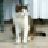
\includegraphics[height=4cm, align=c]{../figures/carlini_wagner_orig.pdf} & 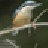
\includegraphics[height=4cm, align=c]{../figures/carlini_wagner_adversarial.pdf} & 
\includegraphics[height=4cm, align=c]{../figures/carlini_wagner_diff.pdf}\\
		\\
		Boundary & 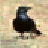
\includegraphics[height=4cm, align=c]{../figures/boundary_orig.pdf} & 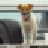
\includegraphics[height=4cm, align=c]{../figures/boundary_adversarial.pdf} & 
\includegraphics[height=4cm, align=c]{../figures/boundary_diff.pdf}\\
		\\
		DeepFool & 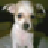
\includegraphics[height=4cm, align=c]{../figures/deepfool_orig.pdf} & 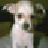
\includegraphics[height=4cm, align=c]{../figures/deepfool_adversarial.pdf} & 
\includegraphics[height=4cm, align=c]{../figures/deepfool_diff.pdf}\\
		\\
		Universal & 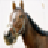
\includegraphics[height=4cm, align=c]{../figures/universal_orig.pdf} & 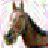
\includegraphics[height=4cm, align=c]{../figures/universal_adversarial.pdf} & 
\includegraphics[height=4cm, align=c]{../figures/universal_diff.pdf}\\
		\\
		\vspace{0.1cm}\\
	\end{tabular}
	\caption{Original images from the CIFAR10 dataset (left), adversarial images (middle) and the corresponding perturbation (right) calculated for a CapsNet.\label{tab:images}}
\end{figure}
\end{block}


\end{column} % End of column 2.2

\end{columns} % End of the split of column 2

\end{column} % End of the second column

\begin{column}{\sepwid}\end{column} % Empty spacer column

\begin{column}{\onecolwid} % The third column


\begin{block}{Conclusion}

Our experiments show that CapsNets are not in general more robust to
white-box attacks. With sufficiently sophisticated attacks CapsNets
can be fooled as easily as ConvNets.  Moreover, we showed that adversarial examples can be transferred
between the two architectures. To fully understand the possibly distinguishable roles of the convolutional and capsule layers with respect to adversarial attacks, we are currently examining the effects of attacks on the activation level of single neurons.  However, this analysis is not finished yet and beyond the scope of this paper.

\end{block}

\begin{block}{References}

%\nocite{*} % Insert publications even if they are not cited in the poster
\tiny{\bibliographystyle{unsrt}
\bibliography{icml}\vspace{0.75in}}

\end{block}

\setbeamercolor{block title}{fg=red,bg=white} % Change the block title color

\setbeamercolor{block alerted title}{fg=black,bg=norange} % Change the alert block title colors
\setbeamercolor{block alerted body}{fg=black,bg=white} % Change the alert block body colors

\begin{alertblock}{Contact Information}

\begin{itemize}
%\item Web: \href{https://www.cs.hhu.de/en/research-groups/machine-learning.html}{https://www.cs.hhu.de/en/research-groups/machine-learning.html}
\item Email: \href{mailto:tobias.uelwer@hhu.de}{tobias.uelwer@hhu.de}  
\item Email: \href{mailto:felix.michels@hhu.de}{felix.michels@hhu.de}
\end{itemize}

\end{alertblock}

%\begin{center}
%\begin{tabular}{ccc}
%\includegraphics[width=0.4\linewidth]{logo.gif} & \hfill & \includegraphics[width=0.4\linewidth]{logo.png}
%\end{tabular}
%\end{center}

%----------------------------------------------------------------------------------------

\end{column} % End of the third column

\end{columns} % End of all the columns in the poster

\end{frame} % End of the enclosing frame

\end{document}
